
% - - - - - - - - - - - - - - - - - - - - - - - - - - - - - -

\begin{frame}
\frametitle{Thinking about Randomness}
  \begin{quote}
    "I, at any rate, am convinced that [God] does not throw dice"
  \end{quote}

  - Albert Einstein 
  \footnote{1926, Letter to Max Born, published in 1971, Irene Born (translator), The Born-Einstein Letters, Walker and Company, New York}
\end{frame}

% - - - - - - - - - - - - - - - - - - - - - - - - - - - - - -

\begin{frame}{Thinking about Randomness}
  \begin{quote}
    "Rational decision makers are able to give reasons for each action they take;
    outside Las Vegas players do not spin roulette wheels"
  \end{quote}

  - Ariel Rubenstein
  \footnote{“John Nash: The Master of Economic Modeling.” The Scandinavian Journal of Economics 97, no. 1 (1995): 9–13. https://doi.org/10.2307/3440824.}
\end{frame}

% - - - - - - - - - - - - - - - - - - - - - - - - - - - - - -

\begin{frame}{Thinking about Randomness}
  
  Why should we use mixed strategies?!
  
  \begin{itemize}
    
    \item As we saw in Activity 2, 
    rarely do real life data fit in completely deterministic models

    \item You can interpret the mixed strategy of one player as the beliefs of other players in equilibrium

    \item Learning some basics of probability theory will help you outside of this class

  \end{itemize}
\end{frame}

% - - - - - - - - - - - - - - - - - - - - - - - - - - - - - -

\begin{frame}
\frametitle{Lotteries}
\begin{itemize}
  \item In this class, any choices with \textit{uncertain} payoffs will be called \alert{lotteries}.
	\item A lottery doesn't have to only be about money
  \item For any set of outcomes in a lottery, there will be an associated probability: if $a$ is a possible outcome, then $P(a)$ is the probability that it occurs.
	\begin{itemize}
		\item All probabilities must be between 0 and 1: $0 \leq P(a) \leq 1$ for all possibilities $a$.
		\item Additionally, the probabilities given in a particular lottery must sum to exactly 1: we will assume that one, and exactly one, outcome must actually occur.
	\end{itemize}
\end{itemize}
\end{frame}

% - - - - - - - - - - - - - - - - - - - - - - - - - - - - - -

\begin{frame}{Expected Utility}
  \begin{itemize}
    \item How can you know how much you like a given lottery
    if you don't even know what the outcome will be?

    \item A natural way would be to think of how happy it would make you \textit{on average}.

    \item The economists' term for this idea is 
    \alert{expected utility} or \alert{expected payoffs}.

  \end{itemize}
\end{frame}

% - - - - - - - - - - - - - - - - - - - - - - - - - - - - - -

\begin{frame}
\frametitle{Expected Payoffs}
\begin{itemize}
  \item You calculate an average by adding up the values of a lottery times the probability of how likely each is.
	\begin{itemize}
    \item $U(a) = \mathbb{E}[u(a)] = \sum_{a}u(a)P(a)$
	\end{itemize}
	\item This is a weighted average of the payoffs associated with each outcome $a$, with the weights being the probabilities of each one happening.
\end{itemize}
\end{frame}

% - - - - - - - - - - - - - - - - - - - - - - - - - - - - - -

\begin{frame}{Double or Nothing 'game'}
  \begin{figure}
    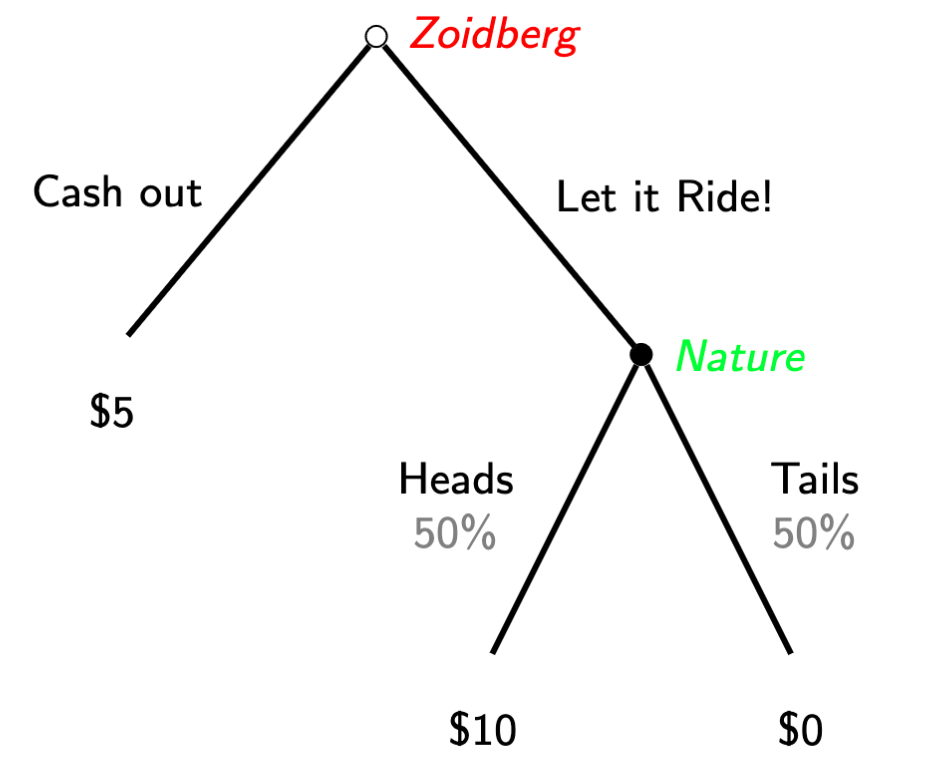
\includegraphics[width = .8\textwidth]{figures/doubleornothing.png}
  \end{figure}
\end{frame}

% - - - - - - - - - - - - - - - - - - - - - - - - - - - - - -

\begin{frame}
\frametitle{Expected Payoff Examples}
\begin{itemize}

  \item Zoidberg's expected payout if he Lets it Ride is 
	$0.50(\$10) + 0.50(\$0) = \$5 - \$0 = \$5$.

  \bigskip
	\item Let's face it, Zoidberg always has luck stacked against him, so suppose instead the coin has a 75\% probability of tails,
  \item The expected payoff would then be $0.25(\$10) + 0.75(\$0) = \$2.50 + \$0 = \$2.50 $.
\end{itemize}
\end{frame}

% - - - - - - - - - - - - - - - - - - - - - - - - - - - - - -

\begin{frame}{Expected Payoff Examples}
  Suppose you roll a fair die and your opponent flips a fair coin simultaneously (independent events).
  You win \$4 whenever a Head appears and the number of dots on the top face of the dice is either one or six. 
  For all other outcomes, you lose \$1. (Dr Rui Zhao, University at Albany)
  \begin{itemize}
    \item How many possible outcomes are there?
    \vspace{5mm}
    \item What is your expected payoff?
    \vspace{5mm}
    \item What is you opponent's expected payoff? 
    Is the game in your favor?
  \end{itemize}
\end{frame}
 
% - - - - - - - - - - - - - - - - - - - - - - - - - - - - - -

\begin{frame}
\frametitle{Test Your Understanding}
\begin{itemize}
	\item Suppose that you like sunny weather, and so you get payoff 5 when it is sunny, and -5 when it is rainy. There is a 10\% chance of rain and a 90\% chance of sun tomorrow. What is the expected payoff of this lottery?
	\begin{enumerate}
		\item -4.5
		\item -4
		\item 0
		\item 4
		\item 4.5
	\end{enumerate}
\end{itemize}
\end{frame}

% - - - - - - - - - - - - - - - - - - - - - - - - - - - - - -

\begin{frame}
\frametitle{Test Your Understanding}
\begin{itemize}
\item Suppose that in addition to a payoff of 5 when it is sunny and -5 when it is rainy, you get a payoff of 2 when it is overcast. There is a 40\% chance of rain, a 40\% chance of overcast, and a 20\% chance of sun tomorrow. What is the expected payoff of this lottery?
\begin{enumerate}
	\item -1.2
	\item -0.2
	\item 0
	\item 0.2
	\item 1.2
\end{enumerate}
\end{itemize}
\end{frame}

% - - - - - - - - - - - - - - - - - - - - - - - - - - - - - -

\begin{frame}
\frametitle{Cardinal Payoffs}
\begin{itemize}
\item Using expected payoffs implies that the payoffs of the outcomes are \alert{cardinal}, not merely ordinal: this means that the payoffs can be used not just to rank, but to compare the relative ``goodness" of outcomes.
\begin{itemize}
	\item i.e. an outcome with payoff 2 is actually twice as good as an outcome with payoff 1.
\end{itemize}
\end{itemize}
\end{frame}

\begin{frame}{Von-Neumann Morgenstern Utility}

  There are a few other axioms beyond just \textit{completeness} and \textit{transitivity}
  which are needed when it comes to making rational choices over lotteries.

  \begin{itemize}
    \item \alert{Continuity:} Small changes in lottery probabilities shouldn't make your ranking jump around.
    \item \alert{Independence:} If you know which of two lotteries you prefer, when I add a little bit of another unrelated option into both, it shouldn't change your mind.
  \end{itemize}

  Because \textit{expected utility} requires special assumptions beyond those of regular \textit{utility}, 
  it gets it's own special name: \\
  \alert{Von-Neumann Morgenstern utility function}
\end{frame}
% - - - - - - - - - - - - - - - - - - - - - - - - - - - - - -

\begin{frame}
\frametitle{Types of Uncertainty}
\begin{itemize}
	\item There are two main types of uncertainty that we'll cover in this course: \alert{external} and \alert{internal}.
  \item \alert{External uncertainty} results from factors outside of the game that the players don't control, such as weather or other random events.
  \item \alert{Internal uncertainty} result from players' own actions inside of the game: it is caused whenever a player acts in a random way.
\end{itemize}
\end{frame}

% - - - - - - - - - - - - - - - - - - - - - - - - - - - - - -

\begin{frame}
\frametitle{External Uncertainty: States of Nature}
\begin{itemize}
\item The simplest form of uncertainty that we'll discuss is \underline{simple uncertainty}, or uncertainty about the \underline{state of nature}.
\item Players don't know which state of nature will occur --- 
  but we assume that they do \textit{know the probability associated with each state}.
\end{itemize}
\end{frame}

% - - - - - - - - - - - - - - - - - - - - - - - - - - - - - -

\begin{frame}
\frametitle{Example: A Card Game}
\begin{itemize}
\item There are two players, Doc and Wyatt. Both are dealt a hand of cards:
  there is a 50\% probability that Wyatt's hand is better,
  and a 50\% probability that Doc's is. 
  There are no ties.
\item At the beginning of the game, both players must bet \$1. 
\item After seeing his cards, Doc may either Stay, keeping the \$1 bet, or may Raise, bringing his bet to \$2.
\item Doc simultaneously decides to either Match Doc's bet, whatever that may be, or to Quit and forfeit his \$1.
\item If Wyatt Matches, the player with the better hand wins all the money. If Wyatt Quits, Doc wins all the money by default.
\end{itemize}
\end{frame}

% - - - - - - - - - - - - - - - - - - - - - - - - - - - - - -

\begin{frame}
\frametitle{Game Table: Doc's Hand is Better}
\begin{itemize}
\item In the state of nature where Doc has the better hand, this is the game table:
\end{itemize}
\begin{table}[h]
\centering

\begin{tabular}{cc|c|c|}
& \multicolumn{1}{c}{} & \multicolumn{2}{c}{Wyatt}\\
& \multicolumn{1}{c}{} & \multicolumn{1}{c}{$Match$}  & \multicolumn{1}{c}{$Quit$} \\\cline{3-4}
\multirow{2}*{Doc}  & $Stay$ & $1, -1$ & $1, -1$ \\\cline{3-4}
& $Raise$ & $2, -2$ & $1,-1$ \\\cline{3-4}
\end{tabular}
\end{table}
\end{frame}

% - - - - - - - - - - - - - - - - - - - - - - - - - - - - - -

\begin{frame}
\frametitle{Game Table: Wyatt's Hand is Better}
\begin{itemize}
\item On the other hand, if Wyatt has the better hand, this is the game table:
\end{itemize}
\begin{table}[h]
\centering
 
\begin{tabular}{cc|c|c|}
& \multicolumn{1}{c}{} & \multicolumn{2}{c}{Wyatt}\\
& \multicolumn{1}{c}{} & \multicolumn{1}{c}{$Match$}  & \multicolumn{1}{c}{$Quit$} \\\cline{3-4}
\multirow{2}*{Doc}  & $Stay$ & $-1, 1$ & $1, -1$ \\\cline{3-4}
& $Raise$ & $-2, 2$ & $1,-1$ \\\cline{3-4}
\end{tabular}
\end{table}
\end{frame}

% - - - - - - - - - - - - - - - - - - - - - - - - - - - - - -

\begin{frame}
\frametitle{Payoffs as Lotteries}
\begin{itemize}
\item We could easily solve each of these game tables to find the NE in either state of nature---but that doesn't matter, because neither player knows which state really applies. 
\item Instead, to solve this game, we must approach the payoffs as lotteries:
\begin{itemize}
\item Doc's payoff from ($Stay,~Match$): he gains 1 with probability 0.5, and loses 1 with probability 0.5.
\item Wyatt's payoff from ($Stay,~Match$): he loses 1 with probability 0.5, and gains 1 with probability 0.5.
\item the expected payoffs of these lotteries are both 0. 
\end{itemize}
\item We can find the expected payoffs associated with each other strategy profile in the same way.
\end{itemize}
\end{frame}

% - - - - - - - - - - - - - - - - - - - - - - - - - - - - - -

\begin{frame}
\frametitle{Game Table: Expected Payoffs}
\begin{table}[h]
\centering
 
\begin{tabular}{cc|c|c|}
& \multicolumn{1}{c}{} & \multicolumn{2}{c}{Wyatt}\\
& \multicolumn{1}{c}{} & \multicolumn{1}{c}{$Match$}  & \multicolumn{1}{c}{$Quit$} \\\cline{3-4}
\multirow{2}*{Doc}  & $Stay$ & $0, 0$ & $1, -1$ \\\cline{3-4}
& $Raise$ & $0, 0$ & $1,-1$ \\\cline{3-4}
\end{tabular}
\end{table}
\begin{itemize}
\item It is trivial to see that the Nash equilibria of this game under uncertainty are ($Stay,~Match$) and ($Raise,~Match$).
\end{itemize}
\end{frame}

% - - - - - - - - - - - - - - - - - - - - - - - - - - - - - -


\begin{frame}
\frametitle{Variation: Unknown Probabilities}
\begin{itemize}
\item Suppose that the probability Doc has the better hand is $p$. 
  How large does $p$ have to be before there is a Nash equilibrium where Wyatt Quits?
\begin{itemize}
	\item We can find the expected payoffs in terms of p:
	\item (Stay, Match):
	\begin{itemize}
		\item Doc's Expected Payoff:
    \vspace{10mm}
		\item Wyatt's Expected Payoff:
    \vspace{10mm}
	\end{itemize}
\end{itemize}
\end{itemize}
\end{frame}

% - - - - - - - - - - - - - - - - - - - - - - - - - - - - - -

\begin{frame}
\frametitle{Variation: Unknown Probabilities}
\begin{itemize}
	\item (Raise, Match):
	\begin{itemize}
		\item Doc's Expected Payoff:
    \vspace{10mm}
		\item Wyatt's Expected Payoff:
    \vspace{10mm}
	\end{itemize}
	\item (Stay, Quit) and (Raise, Quit):
  \vspace{10mm}
\end{itemize}
\end{frame}

% - - - - - - - - - - - - - - - - - - - - - - - - - - - - - -

\begin{frame}
\frametitle{Variation: Unknown Probabilities}
\begin{table}[h]
\centering
\begin{tabular}{cc|c|c|}
& \multicolumn{1}{c}{} & \multicolumn{2}{c}{Wyatt}\\
& \multicolumn{1}{c}{} & \multicolumn{1}{c}{$Match$}  & \multicolumn{1}{c}{$Quit$} \\\cline{3-4}
\multirow{2}*{Doc}  & $Stay$ & $2p - 1, 1 - 2p$ & $1, -1$ \\\cline{3-4}
& $Raise$ & $4p - 2, 2 - 4p$ & $1,-1$ \\\cline{3-4}
\end{tabular}
\end{table}
\begin{itemize}
\item If Wyatt Quits, Doc doesn't care whether he Stays or Raises---he gets 1 either way. To have a NE where Wyatt Quits, we just need Wyatt to be happy with Quitting.
\item ($Stay,~Quit$) is a NE if $-1 \geq 1 - 2p$, i.e. if $p \geq 1$.
\item ($Raise,~Quit$) is a NE if $-1 \geq 2 - 4p$, i.e. if $p \geq \frac{3}{4}$.
\item One interpretation of this is that it is only rational for Wyatt to Quit if he is very confident that Doc has the better hand.
\end{itemize}
\end{frame}

% - - - - - - - - - - - - - - - - - - - - - - - - - - - - - -

\begin{frame}
\frametitle{Variation: Sequential Moves}
\begin{itemize}
\item It's not realistic to have Doc and Wyatt move at the same time: in actual card games, Doc would decide whether to raise, and Wyatt would then see that move and decide whether to match or quit.
\item So let's model this as an extensive-form game and make a game tree:
\end{itemize}
\end{frame}

\begin{frame}
\frametitle{Sequential Card Game Tree}
% \begin{figure}
% \centering
% \includegraphics[width=\textwidth]{Images/08SequentialCards.png}
% \end{figure}
\end{frame}

\begin{frame}
\frametitle{Information Sets in the Sequential Card Game}
\begin{itemize}
\item The dashed lines in this game tree denote information sets, showing that neither player knows the state of nature---however, Wyatt does know whether Doc chose to Stay or Raise.
\item When Doc and Wyatt reach one of their information sets, they don't know which of its nodes they're actually at, but in this case, because the node is determined by the state of nature, they know the probabilities of each node.
\item Once again, we can find the expected payoffs associated with each strategy profile. In fact, they're the same payoffs that we had in the strategic-form game---we just need to fit them into a game tree.
\end{itemize}
\end{frame}

\begin{frame}
\frametitle{Expected Payoff Game Tree}
% \begin{figure}
% \centering
% \includegraphics[width=\textwidth]{Images/08SequentialCardsVNM.png}
% \end{figure}
\end{frame}

\begin{frame}
\frametitle{SPNE in the Sequential-Move Card Game}
\begin{itemize}
	\item Let's look for SPNEs in this game---they will depend on what p is.
	\item A good place to start is with \alert{indifference points}, or values of p that make the players indifferent between their choices. Let's look at Wyatt's decisions:
	\begin{itemize}
		\item In the left-hand subgame (after Doc Stays), Wyatt has the choice between $1 - 2p$ and $-1$. Indifference implies that $1 - 2p = -1$, or $p = 1$. Wyatt is only indifferent here if Doc is guaranteed to have the better hand; if $p < 1$, Wyatt will simply prefer to Match.
		\item In the right-hand subgame (after Doc Raises), $2 - 4p = -1$ implies $p = \frac{3}{4}$. If $p < \frac{3}{4}$, Wyatt will prefer to Match; if $p > \frac{3}{4}$, Wyatt will prefer to Quit.
	\end{itemize}
	\item It may help to plot this on a number line...
\end{itemize}
\end{frame}

\begin{frame}
\frametitle{SPNE in the Sequential-Move Card Game}
\begin{itemize}
	\item Now let's consider Doc's decisions:
	\begin{itemize}
		\item If Wyatt plays (Match, Match), implying that $p \leq \frac{3}{4}$, Doc's choice is between $2p-1$ and $4p-2$. Doc is indifferent when $p = \frac{1}{2}$; when p is smaller, he prefers to Stay, and when p is larger, he prefers to Raise.
		\item If Wyatt plays (Match, Quit), implying that $\frac{3}{4} \leq p \leq 1$, Doc's choice is between $2p - 1$ and $1$. Doc is indifferent if $p = 1$; for $\frac{3}{4} \leq p < 1$, Doc prefers to Raise.
		\item If Wyatt plays (Quit, Quit), which he would only do if $p = 1$ exactly, Doc's choice is between $-1$ and $-1$: not really a choice at all. Doc is completely indifferent here.
	\end{itemize}
\end{itemize}
\end{frame}

\begin{frame}
\frametitle{Plotting SPNEs}
\end{frame}

\begin{frame}
\frametitle{Summary of SPNE in Sequential-Move Card Game}
\begin{itemize}
\item We can summarize all of the possible SPNEs as follows:
\begin{itemize}
\item \{Stay, (Match, Match)\} is an SPNE if $0 \leq p \leq \frac{1}{2}$.
\item \{Raise, (Match, Match)\} is an SPNE if $\frac{1}{2} \leq p \leq \frac{3}{4}$.
\item \{Raise, (Match, Quit)\} is an SPNE if $\frac{3}{4} \leq p \leq 1$.
\item \{Stay, (Match, Quit)\}, \{Stay, (Quit, Quit)\}, and \{Raise, (Quit, Quit)\} are all SPNEs if $p = 1$.
\end{itemize}
\end{itemize}
\end{frame}

